\chapter{Introducción}

\section{Qué es Arturito R2D2}

Arturito R2D2 es un robot móvil que recorre el pasillo entre dos hileras de limoneros, encuentra los limones con
una cámara, calcula dónde están en el espacio y los cosecha con un brazo articulado. Es el trabajo práctico final del
Grupo~2 para dos materias a la vez:

\begin{itemize}
  \item \textbf{Robótica I} evalúa el \textbf{brazo}: un manipulador RRR (tres articulaciones rotativas) tipo
        uArm / Dobot Magician, con una pinza de dos servos.
  \item \textbf{Robótica II} evalúa el \textbf{robot móvil}: la base con tracción diferencial, los sensores, la
        seguridad, la integración con ROS~2 y la autonomía.
\end{itemize}

\begin{idea}[Objetivo mínimo para aprobar]
El robot \textbf{se mueve}, \textbf{detecta el limón con YOLO}, \textbf{lo localiza en 3D con visión estéreo} y
\textbf{lo agarra} con el brazo. Todo lo demás (GPS, app móvil, clasificación por tamaño, 30 frutos medidos) viene
después de que esto funcione de punta a punta.
\end{idea}

El limón no figura entre las especies de la guía de Robótica~II, pero su uso fue aprobado por el profesor. También
se aprobó que la herramienta sea una \textbf{pinza con agarre, tracción y giro} en vez de la ventosa de succión que
proponía la consigna.

\begin{figure}[H]
  \centering
  \begin{subfigure}{0.32\textwidth}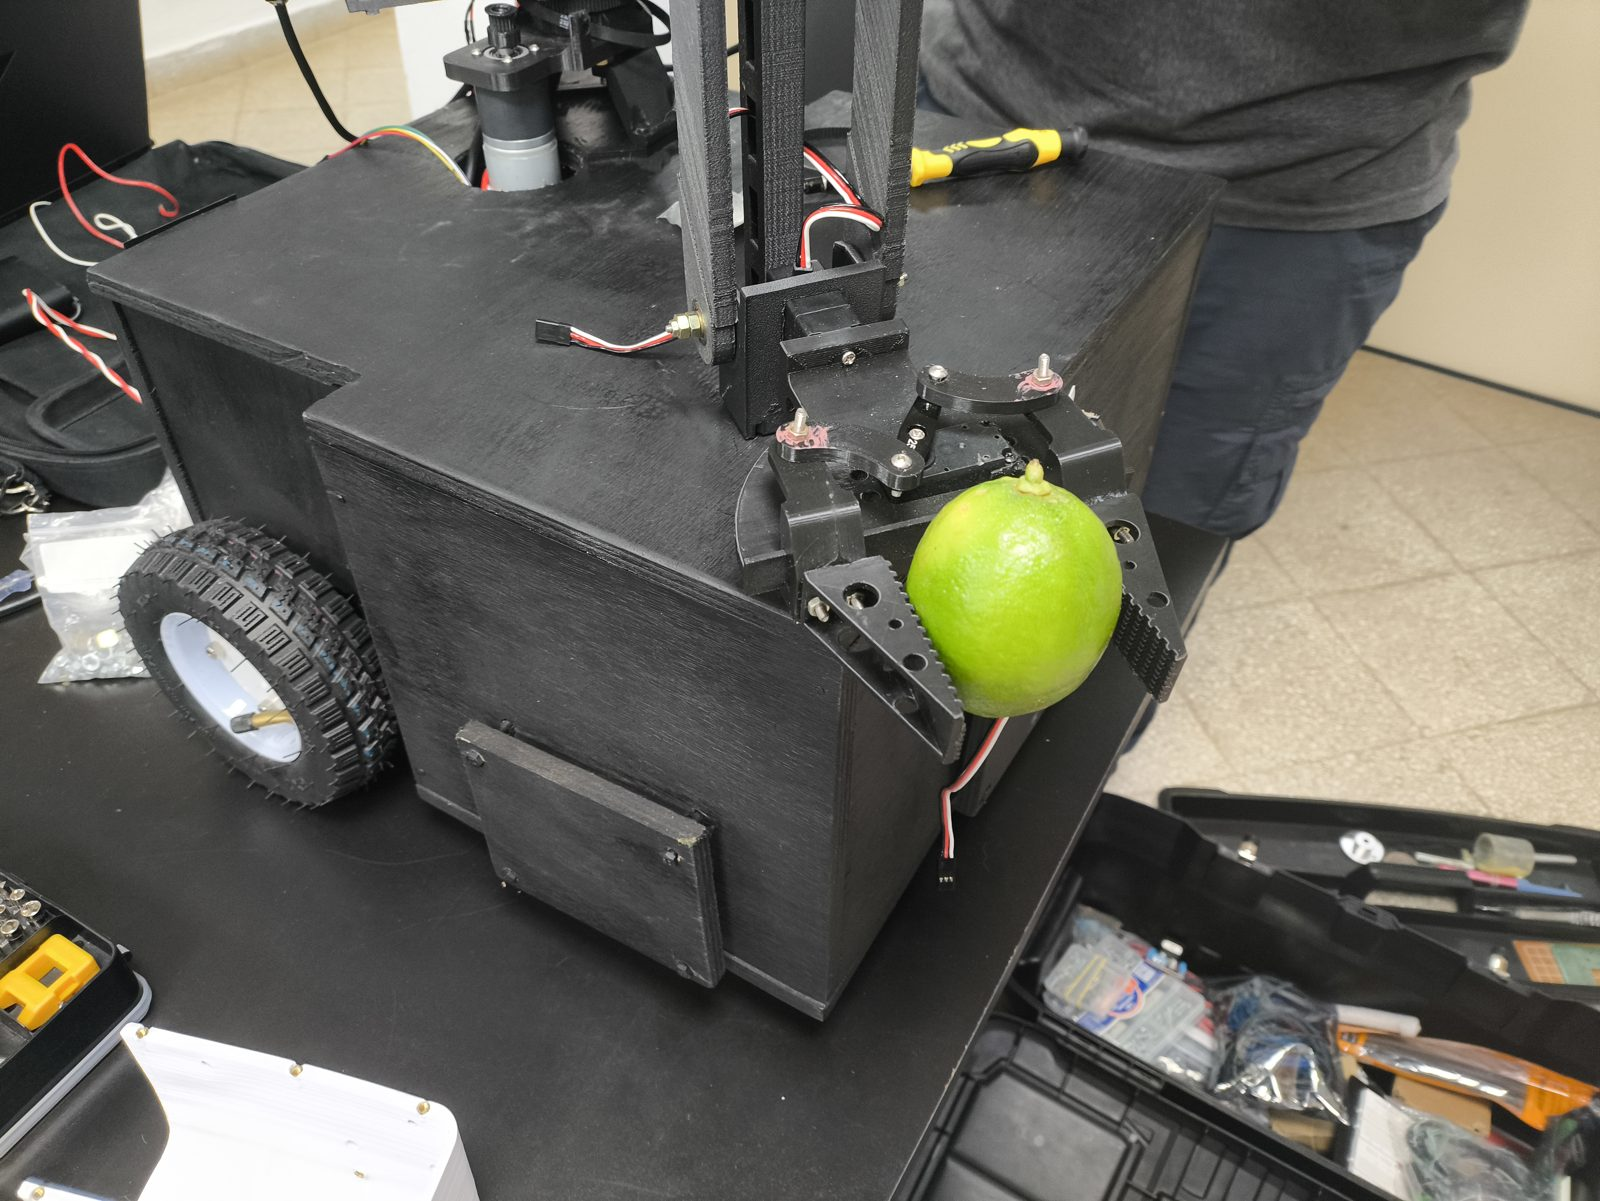
\includegraphics[width=\linewidth]{robot_limon.jpg}\caption{Agarrando un limón.}\end{subfigure}\hfill
  \begin{subfigure}{0.32\textwidth}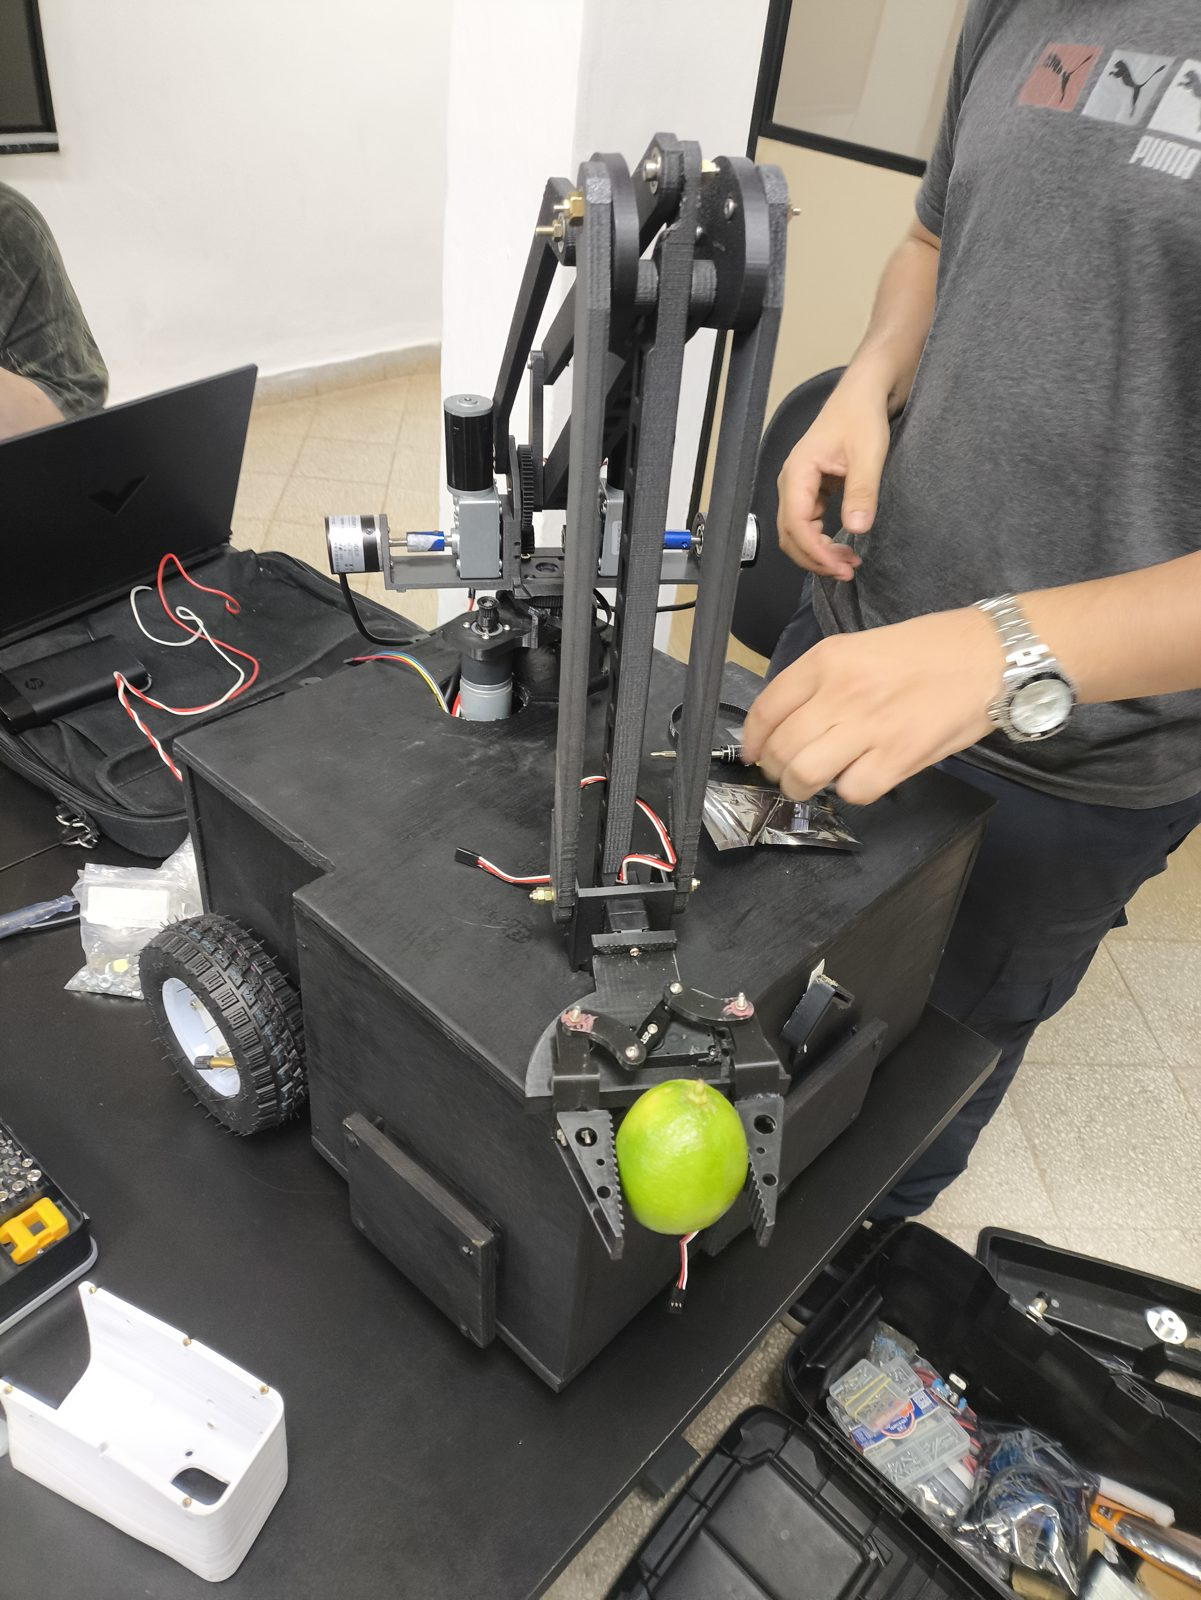
\includegraphics[width=\linewidth]{robot3.jpg}\caption{Brazo sobre la base.}\end{subfigure}\hfill
  \begin{subfigure}{0.32\textwidth}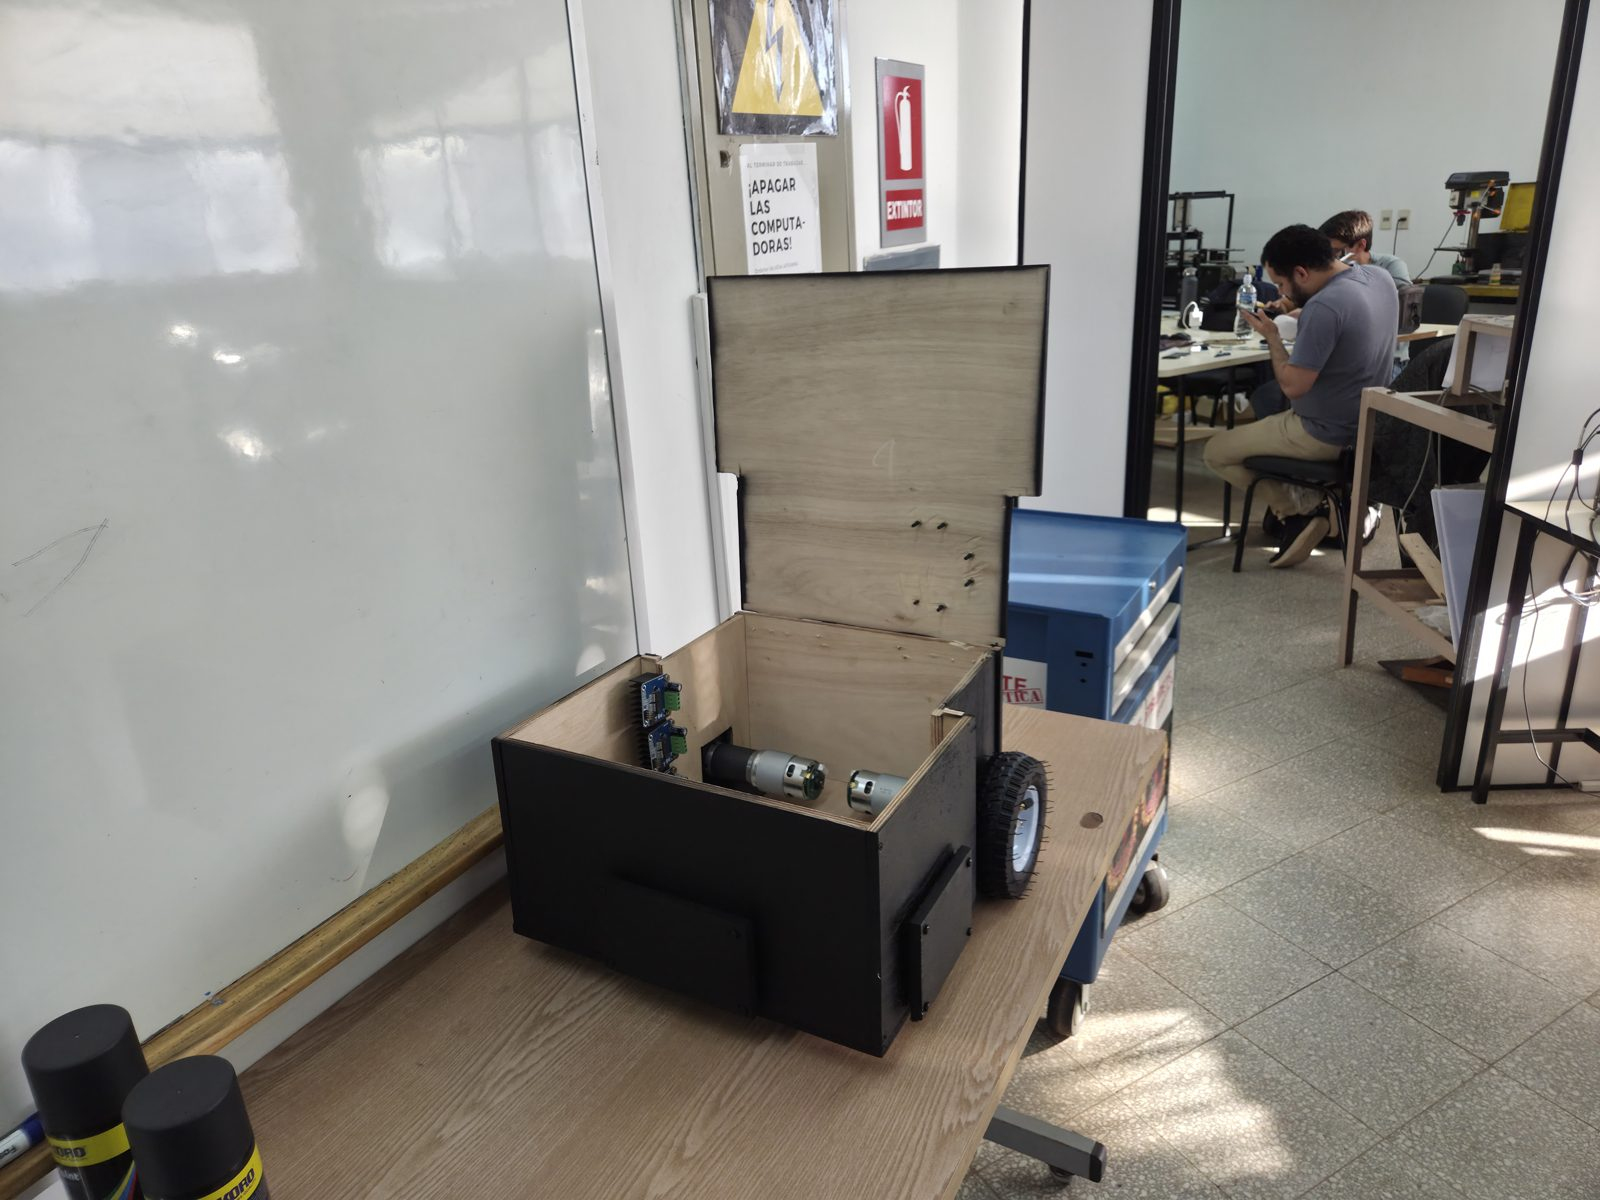
\includegraphics[width=\linewidth]{robot_montado.jpg}\caption{Base de madera en T.}\end{subfigure}
  \caption{El robot en el laboratorio (fotos de las entregas R1~E6 y R2~E3).}
\end{figure}

\section{Cómo leer este manual}

El manual va de lo físico a lo lógico y termina con procedimientos. Se puede leer de corrido o ir directo a lo que
se necesite:

\begin{center}
\begin{tabularx}{\textwidth}{@{}l X@{}}
\toprule
\textbf{Si querés\ldots} & \textbf{Leé} \\
\midrule
Entender el sistema completo en 10 minutos & Capítulo~\ref{cap:general} (vista general) \\
Saber qué es cada pieza física & Capítulos~\ref{cap:mecanica} (mecánica) y \ref{cap:potencia} (potencia) \\
Cablear una placa & Capítulo~\ref{cap:placas} \\
Entender qué hace el código de los ESP32 & Capítulo~\ref{cap:firmware} \\
Aprender ROS~2 desde cero (publicar, suscribir, \textit{launch}) & Capítulo~\ref{cap:ros2} \\
Entender el ``armar'' y cómo hablan la Pi y los ESP32 & Capítulo~\ref{cap:microros} \\
Entender cómo se encuentra el limón en 3D & Capítulo~\ref{cap:vision} \\
Entender cómo se calculan los ángulos del brazo & Capítulo~\ref{cap:ik} \\
Entender cómo decide el robot cuándo frenar y cuánto avanzar & Capítulo~\ref{cap:mision} \\
Probar todo sin hardware & Capítulo~\ref{cap:sim} (Gazebo) \\
Encender el robot por primera vez, paso a paso & Capítulo~\ref{cap:marcha} \\
Arreglar algo que no anda & Capítulo~\ref{cap:diag} \\
Saber qué falta & Capítulo~\ref{cap:estado} \\
Buscar un tópico, un comando o un parámetro & Apéndice~\ref{ap:ref} \\
\bottomrule
\end{tabularx}
\end{center}

\subsection*{Convenciones}
\begin{itemize}
  \item \topic{/cmd\_vel}: un \textbf{tópico} de ROS~2 (un ``canal'' de mensajes).
  \item \archivo{firmware/base/include/pins.h}: un \textbf{archivo} del repositorio \cod{recolector\_de\_frutas}.
  \item \cod{armar}: un \textbf{comando} o texto que se escribe tal cual.
  \item Unidades del Sistema Internacional en todo ROS~2: metros, radianes, segundos. El firmware del brazo trabaja
        internamente en grados y la capa micro-ROS convierte.
  \item Los valores marcados \textbf{MEDIR} son estimaciones: hay que reemplazarlos por lo medido en el robot real.
\end{itemize}

\begin{nota}[Cajas de este manual]
Las cajas azules son notas; las verdes, resúmenes; las rojas, \textbf{cosas que pueden romper algo o lastimar}; las
naranjas, valores o pruebas que todavía faltan.
\end{nota}

\section{Glosario rápido}

\begin{longtable}{@{}p{3.2cm} p{12.3cm}@{}}
\toprule
\textbf{Término} & \textbf{Qué significa acá} \\
\midrule
\endhead
ROS~2 (Jazzy) & \textit{Robot Operating System}: no es un sistema operativo sino un conjunto de bibliotecas y
  herramientas para que muchos programas (nodos) intercambien mensajes. Corre en la Raspberry Pi. \\
Nodo & Un programa de ROS~2. Ej.: el detector YOLO, la cinemática inversa, la misión. \\
Tópico & Canal con nombre por donde viajan mensajes de un tipo fijo. Ej.: \topic{/cmd\_vel} lleva
  \cod{geometry\_msgs/Twist}. \\
Publicar / suscribir & Mandar mensajes a un tópico / recibirlos. Cualquiera puede publicar o suscribirse. \\
micro-ROS & ROS~2 reducido que corre en un microcontrolador (los ESP32). Necesita un \textbf{agente} en la Pi
  que lo conecte con el resto. \\
Agente micro-ROS & Programa en la Pi que hace de puente entre el ESP32 (por USB serie) y la red de ROS~2. \\
Armar / desarmar & Seguro por sesión de cada ESP32: desarmado no acepta órdenes de movimiento
  (capítulo~\ref{cap:microros}). \\
ESP32-S3 & Microcontrolador de la \textbf{base} (tracción, sensores, seguridad). \\
ESP32-WROOM-32D & Microcontrolador del \textbf{brazo} (J1, J2, J3 y la pinza). \\
IBT-2 (BTS7960) & Puente H de potencia que mueve un motor DC en los dos sentidos. Hay cinco. \\
PWM & Modulación por ancho de pulso: cómo el ESP32 le dice al IBT-2 ``cuánta tensión'' darle al motor. \\
Encoder & Sensor en el eje del motor que cuenta pulsos: dice cuánto y a qué velocidad giró. \\
PCNT & Contador de pulsos por hardware del ESP32: cuenta los pulsos del encoder sin usar la CPU. \\
PID / PI & Controlador que corrige la salida según el error entre lo pedido y lo medido. \\
Odometría & Estimar cuánto avanzó y giró el robot integrando lo que midieron los encoders de las ruedas. \\
IMU & Unidad inercial (MPU-6500): acelerómetro y giróscopo. Da el rumbo y detecta vuelcos. \\
HC-SR04 & Sensor de distancia por ultrasonido (hay tres al frente). \\
Bumper & Microinterruptor que se aprieta al chocar (hay tres: frente e izquierda y derecha). \\
Seta & Botón rojo de parada de emergencia. Corta los 12~V de los motores. \\
Estéreo & Dos cámaras separadas 9~cm: comparando las dos imágenes se calcula la distancia. \\
Disparidad & Cuántos píxeles se corre un punto entre la imagen izquierda y la derecha. Más disparidad = más cerca. \\
YOLO & Red neuronal que encuentra objetos (limones) en una imagen y les dibuja una caja. \\
TF & Sistema de ROS~2 que guarda dónde está cada marco de coordenadas (cámara, brazo, base) respecto de los otros. \\
TCP & \textit{Tool Center Point}: el punto de agarre, entre los dedos de la pinza. \\
IK & Cinemática inversa: dado un punto (x, y, z), calcular los ángulos de J1, J2 y J3. \\
FSM & Máquina de estados finitos: el ``cerebro'' de la misión (ESPERAR, APROXIMAR, AGARRAR\ldots). \\
Watchdog & Temporizador que frena todo si deja de llegar una señal periódica. \\
LiPo 3S & Batería de polímero de litio de 3 celdas en serie (11,1~V nominal). \\
Buck & Convertidor que baja la tensión (12~V a 6~V para los servos). \\
\bottomrule
\end{longtable}
